\chapter{Evaluation}\label{chapter:evaluation}

In this chapter, we evaluate the most promising configurations of our training
method. We train three student models on 1M documents with the best-performing
hyperparameters from Chapter~\ref{chapter:experiments} to show the effects of
long training with our teacher-student method. We evaluate the student models
on six classification and two retrieval tasks. For classification tasks, we consider
three contexts, each having a different amount of available supervised data. We
show how the models' performances change for each context and thus
highlight the advantages and disadvantages of our training method.

\section{Student models}

We focus on the three best-performing variants of our training method from
Chapter~\ref{chapter:experiments}. More specifically, we use the hyperparameters
listed in Table~\ref{table:experiments_final_config}. However, as we train the
student models and the contextual teachers on significantly more data, we label
the models differently to avoid confusion. {\CosineStudent} is trained with an
equal mixture of contextual loss and cosine structural loss, which is masked
out for inputs longer than the structural teacher's maximum context length.
{\MSEStudent} is trained with an equal mixture of contextual loss and a
max-margin MSE structural loss. Finally, {\OnlyMSEStudent} is trained only on
the max-margin MSE structural loss. These models' hyperparameters correspond to
the configurations of \Model{masked-cosine;$\lambda$=0.5},
\Model{mm-MSE;$\lambda$=0.5}, and \Model{only-structural;mm-MSE} from
Table~\ref{table:experiments_final_config}, respectively.

\subsection{Training data}

We compile our training corpus the same as \Dataset{val-500k}. Ultimately, we
want to gauge the performance of our training method using the performance of
the trained student models. So, to have a meaningful baseline, we train the
student models only using Longformer's training data. Without any new training
data, the performance of our student model is dependent only on our training
method. Hence, the performance of the student models is proportional to our
training method's performance.

Following Longformer's approach, we equally sample articles from the English
Wikipedia\footnote{\url{https://huggingface.co/datasets/wikipedia/viewer/20220301.en}}
and documents from the RealNews dataset \citep{zellers2019defending} that have
above 1200 Longformer's tokens. We label the resulting dataset as
\Dataset{train-1M} and display its statistics in
Table~\ref{table:train_data_stats}. \Dataset{train-1M} contains relatively long
documents. The average document has around 1300 tokens, and only 34\% of its
documents can fit into the maximum context length of a vanilla Transformer.
However, as we show in Figure~\ref{fig:train_data_dist}, most documents have
between 0 and 500 tokens or 1200 and 1700 tokens.

\begin{table}
    \centering
\begin{tabular}{lrr}
\toprule
Split & Train & Validation \\
\midrule
Documents & 1 000 000 & 30 000 \\
Tokens & 1.37e+09 & 4.15e+07 \\
Tokens per document & 1375$\pm$1738 & 1382$\pm$1697 \\
SBERT tokens over 384 & 71\% & 71\% \\
SBERT tokens over 512 & 66\% & 67\% \\
\bottomrule
\end{tabular}


    \caption{Statistics of \Dataset{train-1M}. For each split, we also show
    the percentage of documents with the number of SBERT tokens above the given
    threshold.}

    \label{table:train_data_stats}

\end{table}

\begin{figure}
    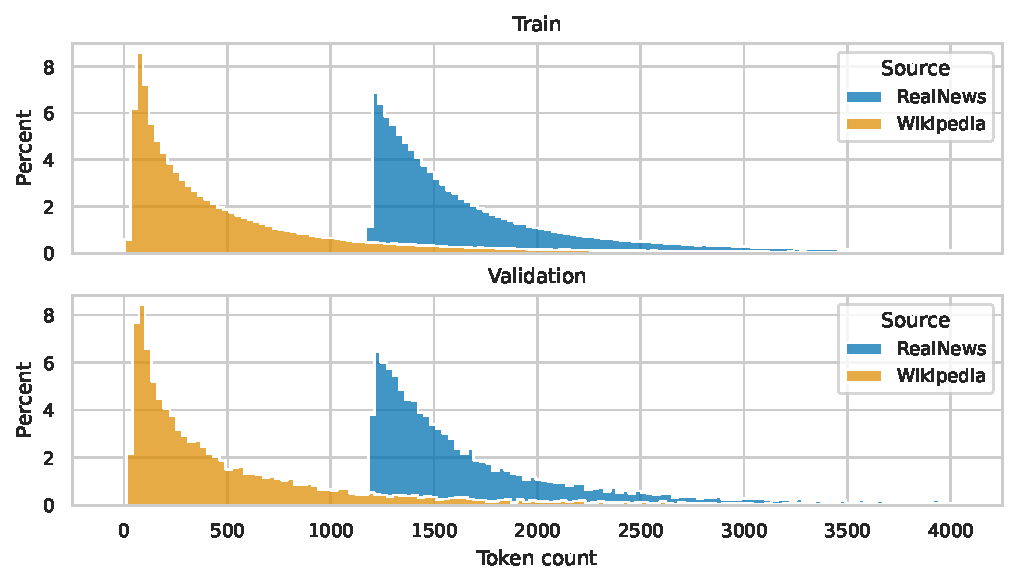
\includegraphics[width=\textwidth]{./img/train_data_dist.pdf}

    \caption{Distribution of the number of Longformer tokens per document in
    \Dataset{train-1M}.}

    \label{fig:train_data_dist}
\end{figure}


\subsection{Training of contextual teachers}

Two of our student models use a contextual teacher. To showcase the full
potential of our training method, we train the contextual teachers anew and
with much more data than in the previous chapter. {\CosineStudent} uses a
2048-dimensional Paragraph Vector \citep{le2014distributed} composed of
Distributed Memory and Distributed Bag of Words models. {\MSEStudent} uses only
a 100-dimensional Distributed Memory model. {\CosineStudent} and {\MSEStudent}
use the best-performing hyperparameters from Section~\ref{section:pv_training}
labelled as \Model{PV;2048d} and \Model{DM;100d} respectively.

We compile the contextual teacher's training dataset in the same manner as
\Dataset{train-1M}. We avoid new data, as the contextual teachers' training
data also becomes the student's training data. Therefore, we restrict the
contextual teachers' training data to Longformer's training data for the
reasons we mention in the previous section. However, as PV is a significantly
smaller model than our student model, we can afford to train it with
substantially more data. We use all available data from RealNews articles and
an equal amount of Wikipedia documents. The resulting dataset has 8.3 million
documents. We label the trained 2048-dimensional and 100-dimensional teachers
\Model{DM} and \Model{PV}. To keep the models' memory footprint manageable, we
restrict \Model{DM}'s vocabulary to $6\times 10^7$ words and \Model{PV}'s
vocabulary to $1.2\times 10^7$ words. With these limitations, the models take
up approximately 96GB and 124GB of memory during prediction.

\subsection{Training of student models}

Finally, we train the student models with the newly trained contextual teachers.
We train on \Dataset{train-1M} for one epoch with hyperparameters listed in
Table~\ref{table:final_student_train_params}. Thanks to the student's efficient
self-attention, the models take up only 12GB of VRAM during training. We train
the models on an NVIDIA A100 GPU card for approximately 30 hours.

\begin{table}
  \centering
  \footnotesize

  \begin{tabular}{l c}
    \toprule
    Parameter & Value \\
    \midrule
    Batch size & 6 \\
    Weight decay & 0.1 \\
    Learning rate & 3e-5 \\
    Learning rate decay & Cosine \\
    Maximum gradient norm & 1.0 \\
    Optimizer & AdamW \\
    Gradient accumulation steps & 10 \\
    Warmup update steps & 500\\
    Gradient checkpointing & Yes \\
    Mixed-precision training & Yes \\
    \bottomrule
  \end{tabular}

  \caption{Hyperparameters used for training all three student models:
  {\CosineStudent}, {\MSEStudent}, and {\OnlyMSEStudent}.}

  \label{table:final_student_train_params}

\end{table}

\section{Evaluation tasks}

We thoroughly evaluate the student models using eight diverse tasks. We
select six classification tasks that cover citation prediction, plagiarism
detection, sentiment, and topic classification. We also include two retrieval
tasks from distinct domains.

We present an overview of the selected classification tasks in
Table~\ref{table:eval_cls_tasks_overview}. Besides ordinary classification
tasks, we also include classifications of pairs of documents. In these tasks,
the classifier bases its prediction on the comparison of two documents, or in
our case,  their two embeddings. As can be seen from
Table~\ref{table:evaluation_tasks_stats}, the amount of the tasks' finetuning
and evaluation data ranges greatly. This becomes particularly important in
Section~\ref{section:eval_cls_tasks}, where we evaluate the student models
while limiting the tasks' training data to different amounts.

\begin{table}
  \footnotesize
  \centering

  \begin{tabular}{llrrr}
      \toprule
      \multicolumn{3}{c}{} & \multicolumn{2}{c}{Class percentage} \\
      \cline{4-5}
      Dataset & Inputs & Classes & Train & Test \\
      \midrule
      \Task{arxiv} & documents & 11 & 9.09$\pm$1.25\% & 9.09$\pm$1.30\% \\
      \Task{imdb} & documents & 2 & 50.00$\pm$0.00\% & 50.00$\pm$0.00\% \\
      \Task{aan} & pairs of documents & 2 & 50.00$\pm$1.50\% & 50.00$\pm$0.77\% \\
      \Task{oc} & pairs of documents & 2 & 50.00$\pm$0.07\% & 50.00$\pm$0.34\% \\
      \Task{pan} & pairs of documents & 2 & 50.00$\pm$0.00\% & 50.00$\pm$0.00\% \\
      \Task{s2orc} & pairs of documents & 2 & 50.00$\pm$0.09\% & 50.00$\pm$0.33\% \\
      \bottomrule
  \end{tabular}

  \caption{Overview of the classification tasks. For each task, we
  include the type of input classified and the mean and standard
  deviation of class percentages.}

  \label{table:eval_cls_tasks_overview}

\end{table}

\begin{table}
  \footnotesize
  \centering
    \begin{tabular}{llrrr}
        \toprule
        & & & \multicolumn{2}{c}{SBERT tokens} \\
        \cline{4-5}
        Dataset & Split & Documents & Over 384 & Over 512 \\
        \midrule
        \multirow[c]{2}{*}{\Task{arxiv}} & Train & 28 388 & 100.00\% & 100.00\% \\
        & Test & 2 500 & 100.00\% & 100.00\% \\
        \cline{1-5}
        \multirow[c]{2}{*}{\Task{imdb}} & Train & 25 000 & 24.56\% & 14.68\% \\
        & Test & 25 000 & 23.54\% & 13.95\% \\
        \cline{1-5}
        \multirow[c]{2}{*}{\Task{aan}} & Train & 106 592 & 0.37\% & 0.06\% \\
        & Test & 13 324 & 0.45\% & 0.08\% \\
        \cline{1-5}
        \multirow[c]{2}{*}{\Task{oc}} & Train & 240 000 & 12.31\% & 1.07\% \\
        & Test & 30 000 & 12.24\% & 1.02\% \\
        \cline{1-5}
        \multirow[c]{2}{*}{\Task{pan}} & Train & 17 968 & 69.93\% & 59.45\% \\
        & Test & 2 906 & 60.82\% & 47.37\% \\
        \cline{1-5}
        \multirow[c]{2}{*}{\Task{s2orc}} & Train & 152 000 & 33.24\% & 18.67\% \\
        & Test & 19 000 & 32.96\% & 18.20\% \\
        \cline{1-5}
        \bottomrule
    \end{tabular}

    \caption{Statistics of the classification tasks. We
    include the percentage of documents with SBERT tokens above a given
    threshold for each task and split.}

    \label{table:evaluation_tasks_stats}

\end{table}

We present an overview of the retrieval tasks in
Table~\ref{table:eval_sims_tasks}. These tasks do not have any finetuning data
and test only the proximity of embeddings of similar documents. Both tasks have
around 90 source articles, each with around eight similar target articles.
However, \Task{games} has substantially more documents.

\begin{table}
  \centering
  \footnotesize
  \begin{tabular}{lrrrrr}
    \toprule
    & & & & \multicolumn{2}{c}{SBERT tokens} \\
    \cline{5-6}
    Dataset & Documents & Sources & Targets per source & Over 384 & Over 512 \\
    \midrule
    \Task{wines} & 1 662 & 89 & 8.92$\pm$1.23 & 100.00\% & 90.43\% \\
    \Task{games} & 21 228 & 88 & 8.74$\pm$2.35 & 100.00\% & 91.78\% \\
    \bottomrule
  \end{tabular}

  \caption{Statistics of our similarity-based evaluation tasks. Each dataset
  has around 90 source documents, each similar to around nine target documents. We
  also include the percentage of documents with SBERT tokens above
  the given threshold.}

  \label{table:eval_sims_tasks}

\end{table}

We pay special attention to the lengths of documents contained in the datasets
and try to cover a span of lengths as large as possible. However, high-quality
long document datasets are very rare due to their annotation's high complexity
and cost. Often, a dataset is said to be composed of documents, but it contains
only shorter pieces of text, such as abstracts. So, we include only one dataset
containing very long documents. As Figure~\ref{fig:eval_tasks_length_dist}
shows, the tasks arguably focus more on documents up to around 1024 tokens.
Nonetheless, as we show in
Tables~\ref{table:evaluation_tasks_stats}~and~\ref{table:eval_sims_tasks} the
tasks still contain a considerable number of documents longer than the maximum
context of our structural teacher.

\begin{figure}

    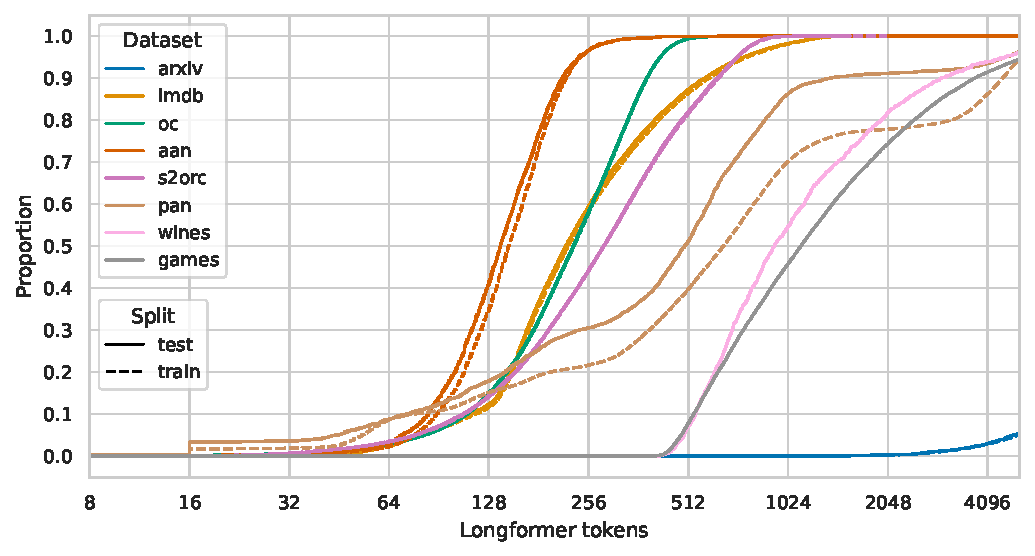
\includegraphics[width=\textwidth]{./img/eval_tasks_token_ecdf.pdf}

    \caption{Estimated cumulative length distribution of the number of
    Longformer tokens in a document.}

    \label{fig:eval_tasks_length_dist}
\end{figure}

\subsection{Tasks' description}

\paragraph{IMDB movie reviews} The IMDB dataset~\citep{maas2011learning}
(denoted as \Task{imdb}) is a binary classification dataset frequently used to
evaluate long-context NLP models~\citep{zaheer2020big, beltagy2020longformer,
le2014distributed}. The dataset consists of movie reviews, each with an
associated rating on a 10-point scale. The reviews that rated the movie with 7
points or higher are classified as positive, and reviews with less than 4
points are classified as negative. There can be up to 30 reviews for each
movie, and the test set contains a disjoint set of movies. Along with the train
and test splits, the dataset contains an unsupervised split without rating or
class labels.

\paragraph{Arxiv papers} Arxiv papers~\citep{arxiv_papers} (denoted as
\Task{arxiv}) is a collection of papers from ArXiv\footnote{\url{arxiv.org}},
an online archive of scholarly papers. Each paper contains its text truncated
to 10000 words but spanning at least 1000 words. The papers are classified into
11 groups based on the scientific field of the given paper. Since each paper
can be associated with several scientific fields, a small portion of the
documents ($\approx$~3.1\%) appear more than once but with different labels.
The scientific fields cover mainly fields of Computer science, such as
Artificial intelligence or Data structures, but also fields connected with
Mathematics, such as Group theory or Statistics theory.

\paragraph{ACL Anthology Network Corpus citations} The ACL Anthology Network
Corpus citations dataset~\citep{zhou2020multilevel} (denoted as \Task{aan}) is
a citation prediction dataset. Each example in the dataset contains a pair of
paper abstracts and is classified as positive if the first document cites the
second one or negative if it does not. The dataset is compiled from the ACL
Anthology Network Corpus~\citep{radev2013acl}, where each source paper creates
positive pairs with all cited papers and a negative pair with one other randomly
sampled non-cited paper.

\paragraph{Semantic Scholar Open Corpus citations} The Semantic Scholar Open
Corpus citations dataset~\citep{zhou2020multilevel} (denoted as \Task{oc}) is
also a citation prediction dataset in the same format as \Task{aan}. As the
dataset name suggests, it was compiled from the Semantic Scholar Open
Corpus~\citep{bhagavatula2018content}. In this dataset, only a single positive
pair is generated for each source paper, resulting in a much higher count of
unique papers compared to \Task{aan}.

\paragraph{PAN plagiarism detection} The final classification dataset is the
PAN plagiarism detection dataset~\citep{zhou2020multilevel} (denoted as
\Task{pan}). It was constructed from PAN plagiarism alignment
task~\citep{potthast2013overview}, which is a collection of pairs of web
documents, where the sections relevant to plagiarism are humanly annotated both
in the source as well as in the suspicious document. \Task{pan} is a binary
classification task where each document pair is classified as positive or
negative. Positive inputs contain the source's plagiarised section, with a part of
the suspicious document containing the corresponding plagiarised section.
Negative pairs are constructed from the positives by replacing the source's
segment with a different part of the same document that is not annotated as being
plagiarised.

\paragraph{Semantic Scholar Open Research Corpus citations} The Semantic
Scholar Open Research Corpus citations dataset~\citep{zhou2020multilevel}
(denoted as \Task{s2orc}) is our third and final citation prediction dataset.
The source of this dataset is the Semantic Scholar Open Research
Corpus~\citep{lo2019s2orc}, where each paper is divided into sections
connected via links to the papers cited within the given section. This structure is
used to generate positive and negative pairs. A section is paired with an
abstract of a cited paper to create a positive pair or an abstract of
a non-cited paper to create a negative pair.


\paragraph{Wines and Video games Wikipedia articles} Both of our
similarity-based tasks are datasets consisting of Wikipedia articles from two
fields of interest: wines (denoted as \Task{wines}) and video games (denoted
as \Task{games})~\citep{ginzburg2021self}. Each dataset contains around 90
source articles, each associated with around nine similar articles. We find the two
datasets unique as they combine two aspects that are rarely seen together. The
similarities are based on expert human annotations, not proxy measures
such as common citations or outgoing links. Additionally, the documents are
relatively long, with around 90\% of documents being longer than 512 tokens.
While \Task{wines} contains fewer documents and covers fewer topics, the
similarities between a source and a target document are less apparent as it is
often based on a few details mentioned throughout the document.

\section{Results}\label{section:eval_results}

This section evaluates the student models on the previously mentioned tasks. To
put the performance of the student models into context, we compare them to four
baselines. First, to estimate the contribution of our training method, we
compare the students to their base checkpoint, Longformer, with a mean pooling
layer over its last hidden states. We also include the performances of the two
contextual teachers \Model{PV} and \Model{DM} and the structural teacher SBERT.
These models showcase the potential of our method. Ideally, we would like the
student models to combine knowledge from all their teachers and surpass all of
them. We evaluate all embedding models without any finetuning. With finetuning
on each task, the models' performance also depends on the used finetuning
method, which makes it more difficult to estimate the contribution of our
training method.

As a classifier, we use a heavily regularized neural network. We train the
classifier with cross-entropy loss for several epochs. We list the complete
list of training hyperparameters in Table~\ref{table:head_train_eval_params}.
We assess the performance of a model based on micro or binary accuracy,
depending on the number of classes. We use micro-averaging for tasks with more
classes to give each input the same weight. When we compare embedding models
across several tasks, we use \emph{normalized accuracy}, which we define in
Section~\ref{section:validation_tasks}.

\begin{table}
  \footnotesize
  \centering

  \begin{tabular}{l c}
    \toprule
    Parameter & Value \\
    \midrule
    Hidden features & 50 \\
    Hidden dropout rate & 0.5 \\
    Hidden activation & ReLU \\
    Epochs & 10 \\
    Batch size & 32 \\
    Weight decay & 0.1 \\
    Label smoothing & 0.1 \\
    Learning rate & 1e-4 \\
    Learning rate decay & Cosine \\
    Maximum gradient norm & 1.0 \\
    Optimizer & AdamW \\
    Mixed-precision training & Yes \\
    \bottomrule
  \end{tabular}

  \caption{Training parameters of classification heads during evaluation.}

  \label{table:head_train_eval_params}

\end{table}

We evaluate the classification tasks in three rounds. In each round, we limit
the number of documents on which the classifier is trained. We find that
evaluating the student models in all three contexts presents a more detailed
picture of the students' performances and highlights the advantages and
disadvantages of our training method. In the first round, we limit the
finetuning documents to 1 thousand. With so few finetuning documents, the
features that help the classifier predict the correct label must be obvious. In
this setting, models that encode a few main features of their input should
achieve the best results. In the second round, we increase the number of
finetuning documents to 10 thousand. Finally, in the last round, we do not
limit the amount of finetuning data. With more finetuning data, the classifiers
can pick up on more complex features. Therefore, in this context, models that
compress as much information as possible into their embedding should, in
theory, achieve the best results. Contrary to the evaluations in
Chapter~\ref{chapter:experiments}, we do not limit the number of test
documents. Thus, overfitting with less data should be obvious. When truncating
the training splits, we downsample it following its label distribution. So, the
downsampled training splits have almost equal class distribution to the
original split.

For retrieval tasks, we measure the embedding's proximity with cosine distance.
As we do not do any training, we use the whole dataset for evaluation. We
measure the models' performances based on Mean Average Precision (\emph{MAP})
but also present Mean Reciprocal Rank (MRR). While MAP scores the entire
predicted ordering, MRR is more interpretable and can be more important in
scenarios where we only care about the first positive result. When we compare
models across both tasks, we use \emph{normalized MAP}, which is computed
similarly to normalized accuracy.

We show an overview of the models' performances in
Table~\ref{table:final_evals}.

\begin{table}
  \begin{subtable}{\textwidth}
    \footnotesize
    \centering
    \begin{tabular}{lrrrrrrrr}
    \toprule
      Model & \Task{arxiv} & \Task{imdb} & \Task{aan} & \Task{oc} & \Task{pan} & \Task{s2orc} & Mean & Norm. mean \\
    \midrule
      Longformer                  &         .649 & \textbf{.913}&         .625 &         .889 &         .675 &         .899 &         .775 &         .894 \\
      \TableModel{DM}             &         .710 &         .731 &         .570 &         .835 &         .685 &         .835 &         .728 &         .843 \\
      \TableModel{PV}             & \textbf{.840}&         .865 &         .703 &         .891 &         .602 &         .899 &         .800 &         .923 \\
      SBERT                       &         .819 &         .890 & \textbf{.805}& \textbf{.935}&         .640 & \textbf{.944}& \textbf{.839}& \textbf{.969}\\
      \TableModel{cosine-masked}  &         .779 &         .843 &         .751 &         .918 &         .638 &         .925 &         .809 &         .935 \\
      \TableModel{MSE-contextual} &         .776 &         .842 &         .767 &         .930 &         .720 &         .942 &         .829 &         .961 \\
      \TableModel{only-MSE}       &         .773 &         .837 &         .760 &         .929 & \textbf{.740}&         .941 &         .830 &         .962 \\
      \midrule
      \multicolumn{9}{c}{10k finetuning documents} \medskip \\
      Longformer                  &         .508 & \textbf{.892}&         .521 &         .742 &         .660 &         .770 &         .682 &         .837 \\
      \TableModel{DM}             &         .650 &         .699 &         .520 &         .683 &         .695 &         .697 &         .657 &         .813 \\
      \TableModel{PV}             & \textbf{.821}&         .852 &         .537 &         .771 &         .585 &         .771 &         .723 &         .885 \\
      SBERT                       &         .785 &         .872 &         .544 &         .787 &         .599 &         .786 &         .729 &         .893 \\
      \TableModel{cosine-masked}  &         .747 &         .821 &         .568 &         .865 &         .629 &         .868 &         .750 &         .918 \\
      \TableModel{MSE-contextual} &         .752 &         .826 & \textbf{.630}&         .886 &         .702 &         .901 &         .783 & \textbf{.963}\\
      \TableModel{only-MSE}       &         .748 &         .821 &         .619 & \textbf{.892}& \textbf{.717}& \textbf{.904}& \textbf{.784}& \textbf{.963}\\
      \midrule
      \multicolumn{9}{c}{1k finetuning documents} \medskip \\
      Longformer                  &         .252 & \textbf{.835}&         .509 &         .655 &         .602 &         .677 &         .588 &         .814 \\
      \TableModel{DM}             &         .215 &         .591 &         .508 &         .567 &         .675 &         .581 &         .523 &         .735 \\
      \TableModel{PV}             &         .640 &         .779 &         .511 &         .654 & \textbf{.677}&         .661 &         .654 &         .918 \\
      SBERT                       &         .606 &         .780 &         .514 &         .601 &         .565 &         .605 &         .612 &         .860 \\
      \TableModel{cosine-masked}  &         .584 &         .726 &         .529 &         .747 &         .658 &         .703 &         .658 &         .922 \\
      \TableModel{MSE-contextual} & \textbf{.645}&         .762 &         .541 & \textbf{.770}&         .629 &         .733 & \textbf{.680}& \textbf{.953}\\
      \TableModel{only-MSE}       &         .642 &         .746 & \textbf{.545}&         .763 &         .635 & \textbf{.750}& \textbf{.680}& \textbf{.953}\\
    \bottomrule
    \end{tabular}

    \caption{Classification tasks}

    \label{table:final_evals_cls}

  \end{subtable}
  \bigskip

  \begin{subtable}{\textwidth}
    \footnotesize
    \centering
    \begin{tabular}{lrrrr}
      \toprule
      Model & \Task{games} & \Task{wines} & Mean & Norm. mean \\
      \midrule
      Longformer                  &         .158 &         .096 &         .127 &         .724 \\
      \TableModel{DM}             &         .130 &         .115 &         .123 &         .717 \\
      \TableModel{PV}             &         .173 &         .133 &         .153 &         .887 \\
      SBERT                       &         .191 &         .143 &         .167 &         .964 \\
      \TableModel{cosine-masked}  &         .165 & \textbf{.148}&         .157 &         .917 \\
      \TableModel{MSE-contextual} &         .186 &         .145 &         .165 &         .957 \\
      \TableModel{only-MSE}       & \textbf{.198}&         .145 & \textbf{.172}& \textbf{.989}\\
      \bottomrule
    \end{tabular}

    \caption{Retrieval tasks}

  \end{subtable}

  \caption{Performance of evaluated embedding models on all downstream tasks.
  For classification tasks, we show the performance on all three rounds,
  revealing the performance with all finetuning data first, then with them
  being limited to 1k and 10k documents. For classification tasks, we show
  binary or micro accuracy. For retrieval tasks, we show MAP. We also display
  the mean score and the mean of normalized scores for each model.}

  \label{table:final_evals}

\end{table}

\subsection{Classification tasks}\label{section:eval_cls_tasks}

We evaluate the embedding models' performance on the classification tasks in
three rounds. First, we compare the overall performance of the models between
the three different rounds. Then, we explore the models' performances per task
in detail.

% - boxplot:
%   - students keep the same relative performance as during validation, but
%   cosine seems to get a bit worse
%     - might be due to significantly less updates caused by structural loss
%   - the relative performance stays the same throughout all rounds
%     - except for: SBERT vs PV in 10k, SBERT vs student models in all
%   - 1k:
%     - students beat baselines
%     - SBERT & Longformer very weak
%     - cosine student just beating its contextual teacher -- demonstrating the
%     small number of structural updates
%   - 10k:
%     - increase in performance all around
%     - students still surpassing all baselines
%     - SBERT now outperforming PV, -- relatively small increase in performance
%     for PV
%     - a bit wider gap between cosine student and mse students
%   - all:
%     - best models get marginally better, worst models catch up -- the
%     differences between models become smaller
%     - SBERT's performance dramatically increases and only just surpasses the
%     best student model -- context not as important, better architecture
%     - the student models still improve the performance set by longformer and
%     both contextual teachers

First, we focus on the overall models' performance throughout the three
evaluation rounds, which we present in Figure~\ref{fig:final_eval_norm_all}.
The relative performance of the baselines and student models is similar to what
we witness in Chapter~\ref{chapter:experiments}. In the first two rounds, the
students outperform all baselines. In the last round, they beat all contextual
teachers and improve the score of Longformer. However, they are only just worse
than SBERT. The best student is {\OnlyMSEStudent} followed by {\MSEStudent}. We
witness the same order of corresponding models on validation tasks at the end
of Chapter~\ref{chapter:experiments}. However, as {\CosineStudent} is trained
with the structural loss only on short inputs, it receives 3.26 times fewer
update steps with the structural loss than the other two students.
Consequently, {\CosineStudent} often outperforms its contextual teacher only by
a fraction, creating a noticeable performance gap between it and the other two
students.

\begin{figure}

  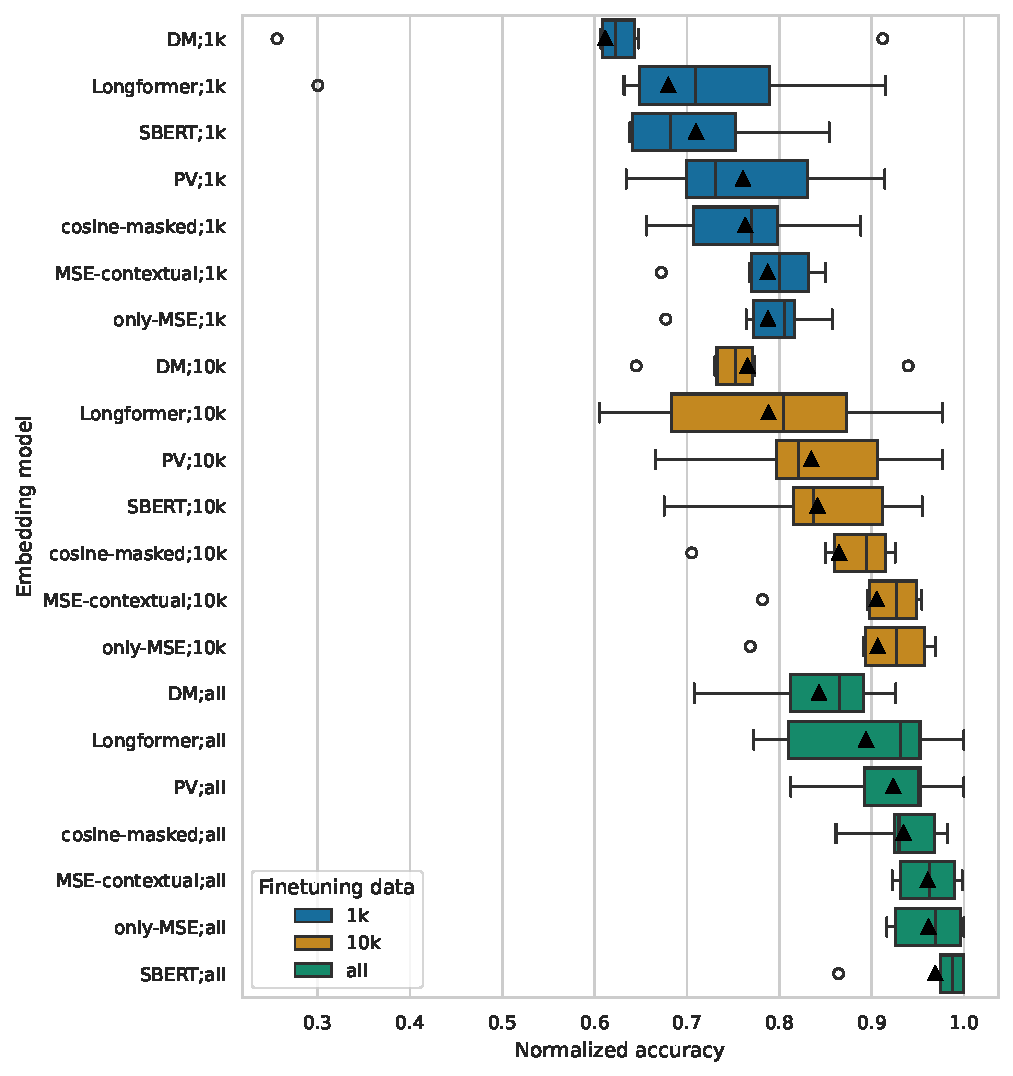
\includegraphics[width=\textwidth]{img/final_eval_norm_all.pdf}

  \caption{Overall relative performance of embedding models throughout the three
  rounds. In the first two rounds, we limit the number of finetuning documents to 1k
  and 10k, but do not set any limit in the third round labeled as ``all''.}

  \label{fig:final_eval_norm_all}

\end{figure}

In the first round, Longformer's and SBERT's performance is underwhelming. At
the same time, the best student model achieves, on average, nearly 80\% of the
best performance for a given task achieved by an embedding model with all
finetuning data. We see this as a considerable achievement since there are 17
to 240 times more finetuning documents in the last round compared to the first
one. In the second round, the classifiers are trained on 10k finetuning
documents, and the performances naturally increase. Particularly for SBERT, as
it now surpasses \Model{PV}, which improves by a relatively small amount. These
effects are also noticeable in the performance of {\CosineStudent} as there is
a more significant gap between it and the other two students that rely more on
SBERT. Finally, with all finetuning data, the differences between models'
performances diminish as the best models improve only marginally. SBERT takes
the greatest advantage of the increase in finetuning data and surpasses all
other models. We see this as a demonstration that the embedding model does not
strictly need a large maximum context for the selected set of tasks. In other
words, despite the moderately large documents, we can reach a competitive
performance by only considering the first 384 tokens of each input. This is
apparent, especially for \Task{arxiv}, where we can imagine classifying the
field of a scholarly paper based on just its abstract. So, as the context is of
minor importance, SBERT benefits from its full attention and surpasses the best
student by a small fraction. Nonetheless, all student models can improve the
scores of their contextual teachers and base checkpoints. Moreover, the
students reach consistent and comparable performances despite being trained
differently. {\CosineStudent} trains with a different contextual teacher,
contextual loss, structural loss, and weighting of the two losses than the rest
of the students. {\MSEStudent} trains with a significantly less performant
contextual teacher, while {\OnlyMSEStudent} does not use a contextual teacher.
This shows that our method is robust and open to multiple changes in various
aspects.


% Per task:
% - SBERT vs students' performances -- the need for context
% - going from 1k to 10k PV got worse on PAN, does it get worse for other tasks as well?
% - 10k DM also (same as PV) surprisingly jumps in performance
% - going from 1k to 10k S2ORC seems to benefit -- what tasks benefit from more finetuning data?
%     - arxiv,
%     - what tasks do not benefit as much: aan, pan
% - Longformer on IMDB
% - from 1k to 10k SBERT jump in perf (small, but consistent):
%    - s2orc, oc, pan, imdb
% - from 1k to 10k for some tasks the differences between students get smaller,
%   for few others they get larger
%     - smaller: arxiv, imdb
%     - larger: pan, aan
%     - same: s2orc, oc
% - from 10k to all:
%   - SBERT jump: aan, s2orc, oc
%   - tasks that benefit: so2rc, oc, aan (for best models)
%       - that do not as much: pan, imdb, arxive
%   - otherwise the relationship between models are pretty much the same:
%     - s2orc, oc, imdb, arxiv, aan, pan
%
%
% What to highlight:
%   - briefly describe tasks and where models do well
%     - well pairs with the "its not about context"
%     - Arxiv not reflecting need for context
%   - go through rounds:
%     - 1k some tasks are very hard
%     - 10k vs final: SBERT capitalizes on aan, s2orc, oc
%   - PV's benefits decrease as we increase the amounts of data (similarly so does students')
%     - on Arxiv, PAN
%
% What to highlight:
%   - SBERT capitalizes most on tasks that have more data
%     - [x] show the figure
%     - [x] SBERT vs student models -- context, arxiv,
%     - [x] PV's performance on Arxiv
%       - not as large improvement with amount of data
%   - Only MSE student and context
%   - [x] Longformer and IMDB

We now examine the models' performances per each task, which we plot in
Figure~\ref{fig:final_cls_evals}. The relative models' performances on a
given task stay consistent throughout the three rounds, so we focus only on the
last two. With 10k finetuning documents, the students perform best on
classifications of document pairs. On \Task{imdb}, Longformer shows the best
performance, which is surprising given it is the second-worst model in both
rounds. On \Task{arxiv}, PV shows the best performance as it benefits from its
large embedding and unlimited context. Arguably, both of these attributes play
a role, as \Model{DM} with the same unlimited context but with more than 50 times smaller embedding performs admirably well but worse than \Model{PV}. As
we increase the number of finetuning documents, SBERT substantially improves.
We register the largest performance increase for tasks with the most
finetuning data available. These are \Task{aan}, \Task{oc}, and \Task{s2orc}.
We also highlight SBERT's performance on \Task{arxiv} in both rounds, where it
outperforms all students with eight times larger maximum context and comes
relatively close to the performance of \Model{PV}. This demonstrates that, despite the task being composed of only very long documents, we can achieve a
competitive performance based on just the first few hundred tokens. The insignificance of an embedding model's lack of context may
partly explain why the students' performances for a given task are not affected by the length of the tasks' documents. For example, on tasks with
longer documents such as \Task{arxiv} or \Task{pan}, {\CosineStudent} and
{\MSEStudent} perform on par with {\OnlyMSEStudent} despite being trained with
a contextual teacher, which should theoretically provide the students with a
larger context.


% With one thousand finetuning documents some tasks are very difficult.
% Especially \Task{aan} with Longformer's or \Model{DM}'s embeddings, where the
% classifiers perform almost as well as a majority classifier. On the other
% hand, \Task{imdb} turns out to be relatively easy, as even with 1k finetuning
% documents Longformer was able to reach 83\% accuracy. That said, Longformer's
% training seems to be unbalanced as it outperforms all models on \Task{imdb},
% despite being the second worst model in all three rounds. These issue do not
% propagate to the student models. With 10k finetuning documents


% As we show in Table~\ref{table:final_evals_cls}, the students are successful
% especially on classifications of document pairs. On \Task{arxiv} \Model{PV}
% shows the strongest performance apart from the first round with the least
% finetuning documents. In the final two rounds, \Model{PV} benefits from its
% large embedding and unlimited context. Arguably, both of these attributes
% play a role, as \Model{DM} with the same unlimited context but with more than
% 50 times smaller embedding performs admirably well but worse than \Model{PV}.
% On \Task{imdb} Longformer consistently reaches the best performance, which is
% surprising since it is the second worst model on 4 out of the 6 tasks. As we
% increase the number of finetuning documents SBERT substantially improves.
% SBERTs increases its per

% If we
% focus separately on each round, we find that with only 1k of finetuning
% documents some tasks turn out to be very difficult. Especially on \Task{aan}
% with Longformer's or \Model{DM}'s embeddings, where the classifiers perform
% almost as well as a majority classifier. As we see in
% Figure~\ref{fig:final_cls_evals}, with 10k finetuning documents

% As we show in Figure~\ref{fig:final_cls_evals}, SBERT is able to surpass all
% other models in the final round thanks to its performance on

% Arguably it is not only thanks to its larger embedding
% but also its unlimited context, since \Model{DM} with more than 50
% times smaller embedding performs admirably well.

% also has an unlimited context and its performance is noticeably
% worse.

% thanks to its unlimited context. its large
% embedding dimension and unlimited context.


% all
% classifiers surpass

% The students' outperform all baselines in \Task{arxiv},
% \Task{aan}, \Task{oc} and \Task{s2orc}.

% by only a fraction.

% With only one thousand documents most classifiers perform poorly.

% We now compare the models' performances per task for the final two rounds in
% Figure~\ref{fig:final_cls_evals}. We also refer to
% Table~\ref{table:final_evals_cls} for exact values.

\begin{figure}

  \centering
  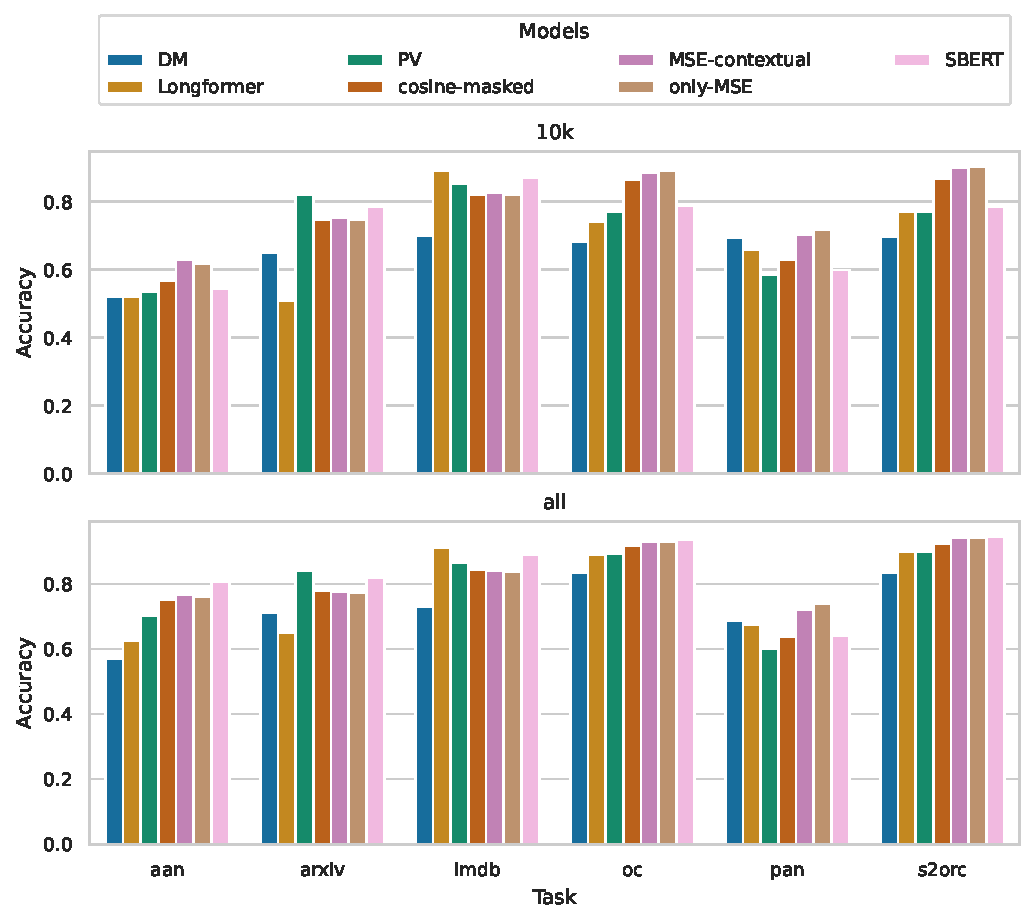
\includegraphics[width=\textwidth]{img/final_cls_evals.pdf}

  \caption{Performance of embedding models on evaluation tasks with and without
  (labeled as ``all'') the train split limited to 10k documents.}

  \label{fig:final_cls_evals}

\end{figure}


%\subsection{With 1k finetuning documents}


%With one thousand finetuning documents, the classifiers have minimum data to
%learn the embeddings' structure. We present overall performance of all student
%models and the baselines in Figure~\ref{fig:1k_norm_evals}. The student models
%outperform both teachers as well as Longformer. The models' relative
%performance is similar to that on validation tasks in
%Chapter~\ref{chapter:experiments}. Using only max-margin MSE structural loss,
%leads to the best results. Adding a contextual loss to the max-margin MSE loss
%hurts the model's performance by a small fraction. With cosine structural loss
%and contextual loss, {\CosineStudent} only just outperforms its contextual
%teacher. We also plot the models' performance by task in
%Figure~\ref{fig:1k_evals}. With only one thousand training documents, some task
%seem to be very hard. Especially for \Task{aan}, and \Task{arxiv} on which some
%classifiers perform only fractionally better than majority class classifier.
%Also the length of documents has little effect on the models' performance.
%SBERT's performance is nearly identical for \Task{arxiv}, \Task{oc} and
%\Task{s2orc}, despite the length distributions of the tasks' documents being
%very dissimilar. In similar fashion, the student's improvement over SBERT's
%does not seem to correspond with the document's length across tasks.

%% Longformer imdb surprise surprise


%\begin{figure}

%  \centering
%  \includegraphics[width=0.85\textwidth]{img/1k_norm_evals.pdf}

%  \caption{Overall performance of embedding models with 1k finetuning
%  documents.}

%  \label{fig:1k_norm_evals}

%\end{figure}

%\begin{figure}

%  \includegraphics[width=\textwidth]{img/1k_evals.pdf}

%  \caption{Performance of embedding models per task with 1k finetuning
%  documents.}

%  \label{fig:1k_evals}

%\end{figure}


%\subsection{With 10k finetuning documents}

%With 10 thousand finetuning documents the classifiers have already a
%substantial amount of data. Again we look first at the relative overall
%performance of the embedding models in Figure~\ref{fig:short_norm_evals}.
%Compared to the models' performances with only 1k of finetuning documents,
%there are only few differences. The student models still surpass all baselines.
%However, SBERT has significantly improved and now outperforms \Model{PV}. Also
%the difference between {\CosineStudent} and the other two students seem to be
%larger. We also plot the models' performances per each task in
%Figure~\ref{fig:short_evals}. The significant increase in finetuning data can
%reveal more performant embeddings. For instance \Model{PV}'s embeddings for
%\Task{arxiv} are surpassing all other models, whereas with only 1k finetuning
%documents they are on par with the students' embeddings. Note that in the case
%of \Task{aan}, \Task{s2orc} or \Task{oc} the students' performances cannot be
%explained by the teachers' or by Longformer's performances as all baselines
%perform worse than all students. This demonstrate how much the students benefit
%from combining knowledge from several other models.

%% unexplicable performance of student models -- no teacher nor the base
%% checkpoint performa as well

%\begin{figure}

%  \centering
%  \includegraphics[width=0.85\textwidth]{img/short_norm_evals.pdf}

%  \caption{Overall performance of embedding models with 10k finetuning
%  documents.}

%  \label{fig:short_norm_evals}

%\end{figure}

%\begin{figure}

%  \includegraphics[width=\textwidth]{img/short_evals.pdf}

%  \caption{Performance of embedding models per task with 10k finetuning
%  documents.}

%  \label{fig:short_evals}

%\end{figure}

%\subsection{With all finetuning data}

%Without limiting the finetuning data, we examine the full performance the
%embedding models can reach. We show the overall performance of all embedding
%models in Figure~\ref{fig:final_norm_evals}. With significantly more finetuning
%data, SBERT's embeddings show remarkable increase in performance. We
%hypothesize, that this is due to a more complex embeddings, whose structure is
%understandable only with larger amounts of data. Since our student models have
%less dense architectures, their ability to generate complex embeddings is not
%as high as SBERT's. Additionally, as we note in the previous sections, the
%embeddings do not seem to benefit from the increased maximum context of the
%student model. Consequently, this suggests that the contextual information is
%not that important for the performance models' in our set of tasks.


%We also plot the models' performances per each task in
%Figure~\ref{fig:final_evals}.


%\begin{figure}

%  \centering
%  \includegraphics[width=0.85\textwidth]{img/final_norm_evals.pdf}

%  \caption{Overall performance of embedding models with all finetuning
%  documents.}

%  \label{fig:final_norm_evals}

%\end{figure}

%\begin{figure}

%  \includegraphics[width=\textwidth]{img/final_evals.pdf}

%  \caption{Performance of embedding models per task with all finetuning
%  documents.}

%  \label{fig:final_evals}

%\end{figure}

\subsection{Retrieval tasks}

We plot the overall models' performances on the retrieval tasks in
Figure~\ref{fig:final_eval_sims}. In terms of MAP, the best-performing model is
{\OnlyMSEStudent} closely followed by SBERT and the other two student models.
For Mean Reciprocal Rank, the best model is {\CosineStudent}, one
of the most consistent models in both metrics. This suggests that using
a structural teacher only for inputs, which it can process as a whole, may lead to a
more consistent student model.

\begin{figure}

  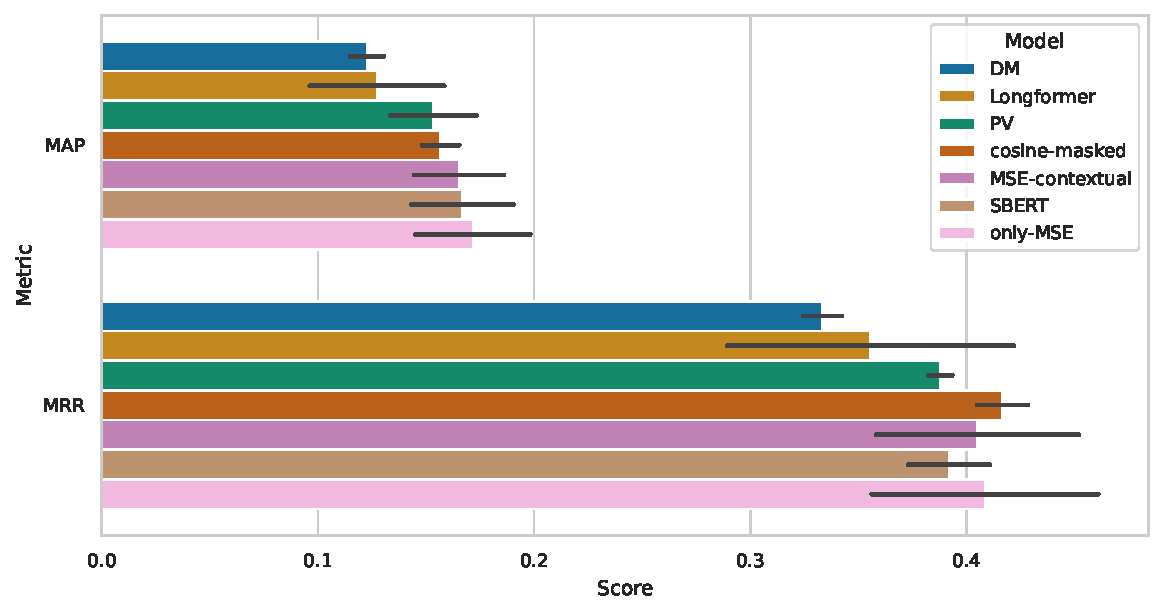
\includegraphics[width=\textwidth]{img/final_sims_evals.pdf}

  \caption{Performance of models on retrieval tasks. We mark the mean score
  with a bar and the span between each task's score with an error bar.}

  \label{fig:final_eval_sims}

\end{figure}

We also plot the models' performances per each task in
Figure~\ref{fig:final_eval_sims_per_task}. As the results suggest, \Task{games}
is an easier task than \Task{wines}. This may be unexpected since, compared to
\Task{wines}, \Task{games} has more total documents but a similar amount of
source and target documents. Consequently, \Task{games} contains much more
``noise'' documents, which may hurt the performance. However, as we mention in
the tasks' description, the selection of topics for \Task{games} is much wider, and the differences between documents are far less nuanced. On the other hand, the
similarities of documents in \Task{wines} are sometimes based on a few details mentioned throughout the document.

\begin{figure}

  \centering
  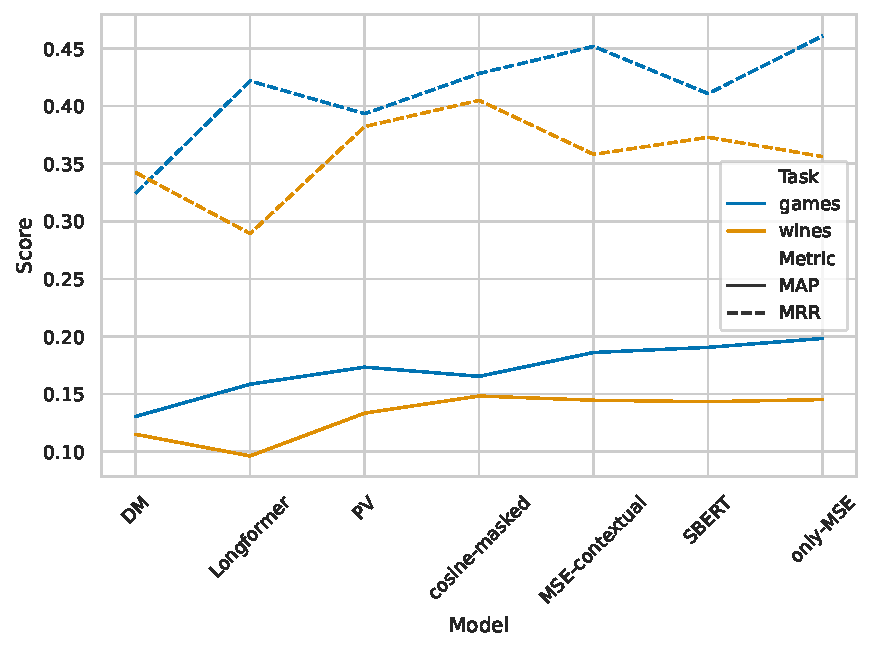
\includegraphics[width=0.85\textwidth]{img/final_sims_evals_per_task.pdf}

  \caption{Performance of embedding models on each retrieval task.}

  \label{fig:final_eval_sims_per_task}

\end{figure}
